%%%%%%%%%%%%%%%%%%%%%%%%%%%%%%%%%%%%%%%%%%%%%%%%%%%%%%%%%%%%%%%%%%%%%%%%%%%%%%%%
%
%   Semester project, fall term 2014
%   Author: Jakob Ehrl, born 01/24/91
%   Study program: Computer science, MA 1
%   
%   Professor Dr. Francesco Mondada
%   Assistant: Dr. Stefan Witwicki
%
%%%%%%%%%%%%%%%%%%%%%%%%%%%%%%%%%%%%%%%%%%%%%%%%%%%%%%%%%%%%%%%%%%%%%%%%%%%%%%%%%

\section{Localization Module}
The localization module is composed of an arduino micro, 6 linear sensor arrays, and a compass. Mounted on a rod in a high position on the robot, it's purpose is to use the geometry of the map, the beacon peaks received by the linear sensor arrays, and the orientation read from the compass in order to triangulate the position and orientation of the robot in the map.

\begin{figure}
\centering
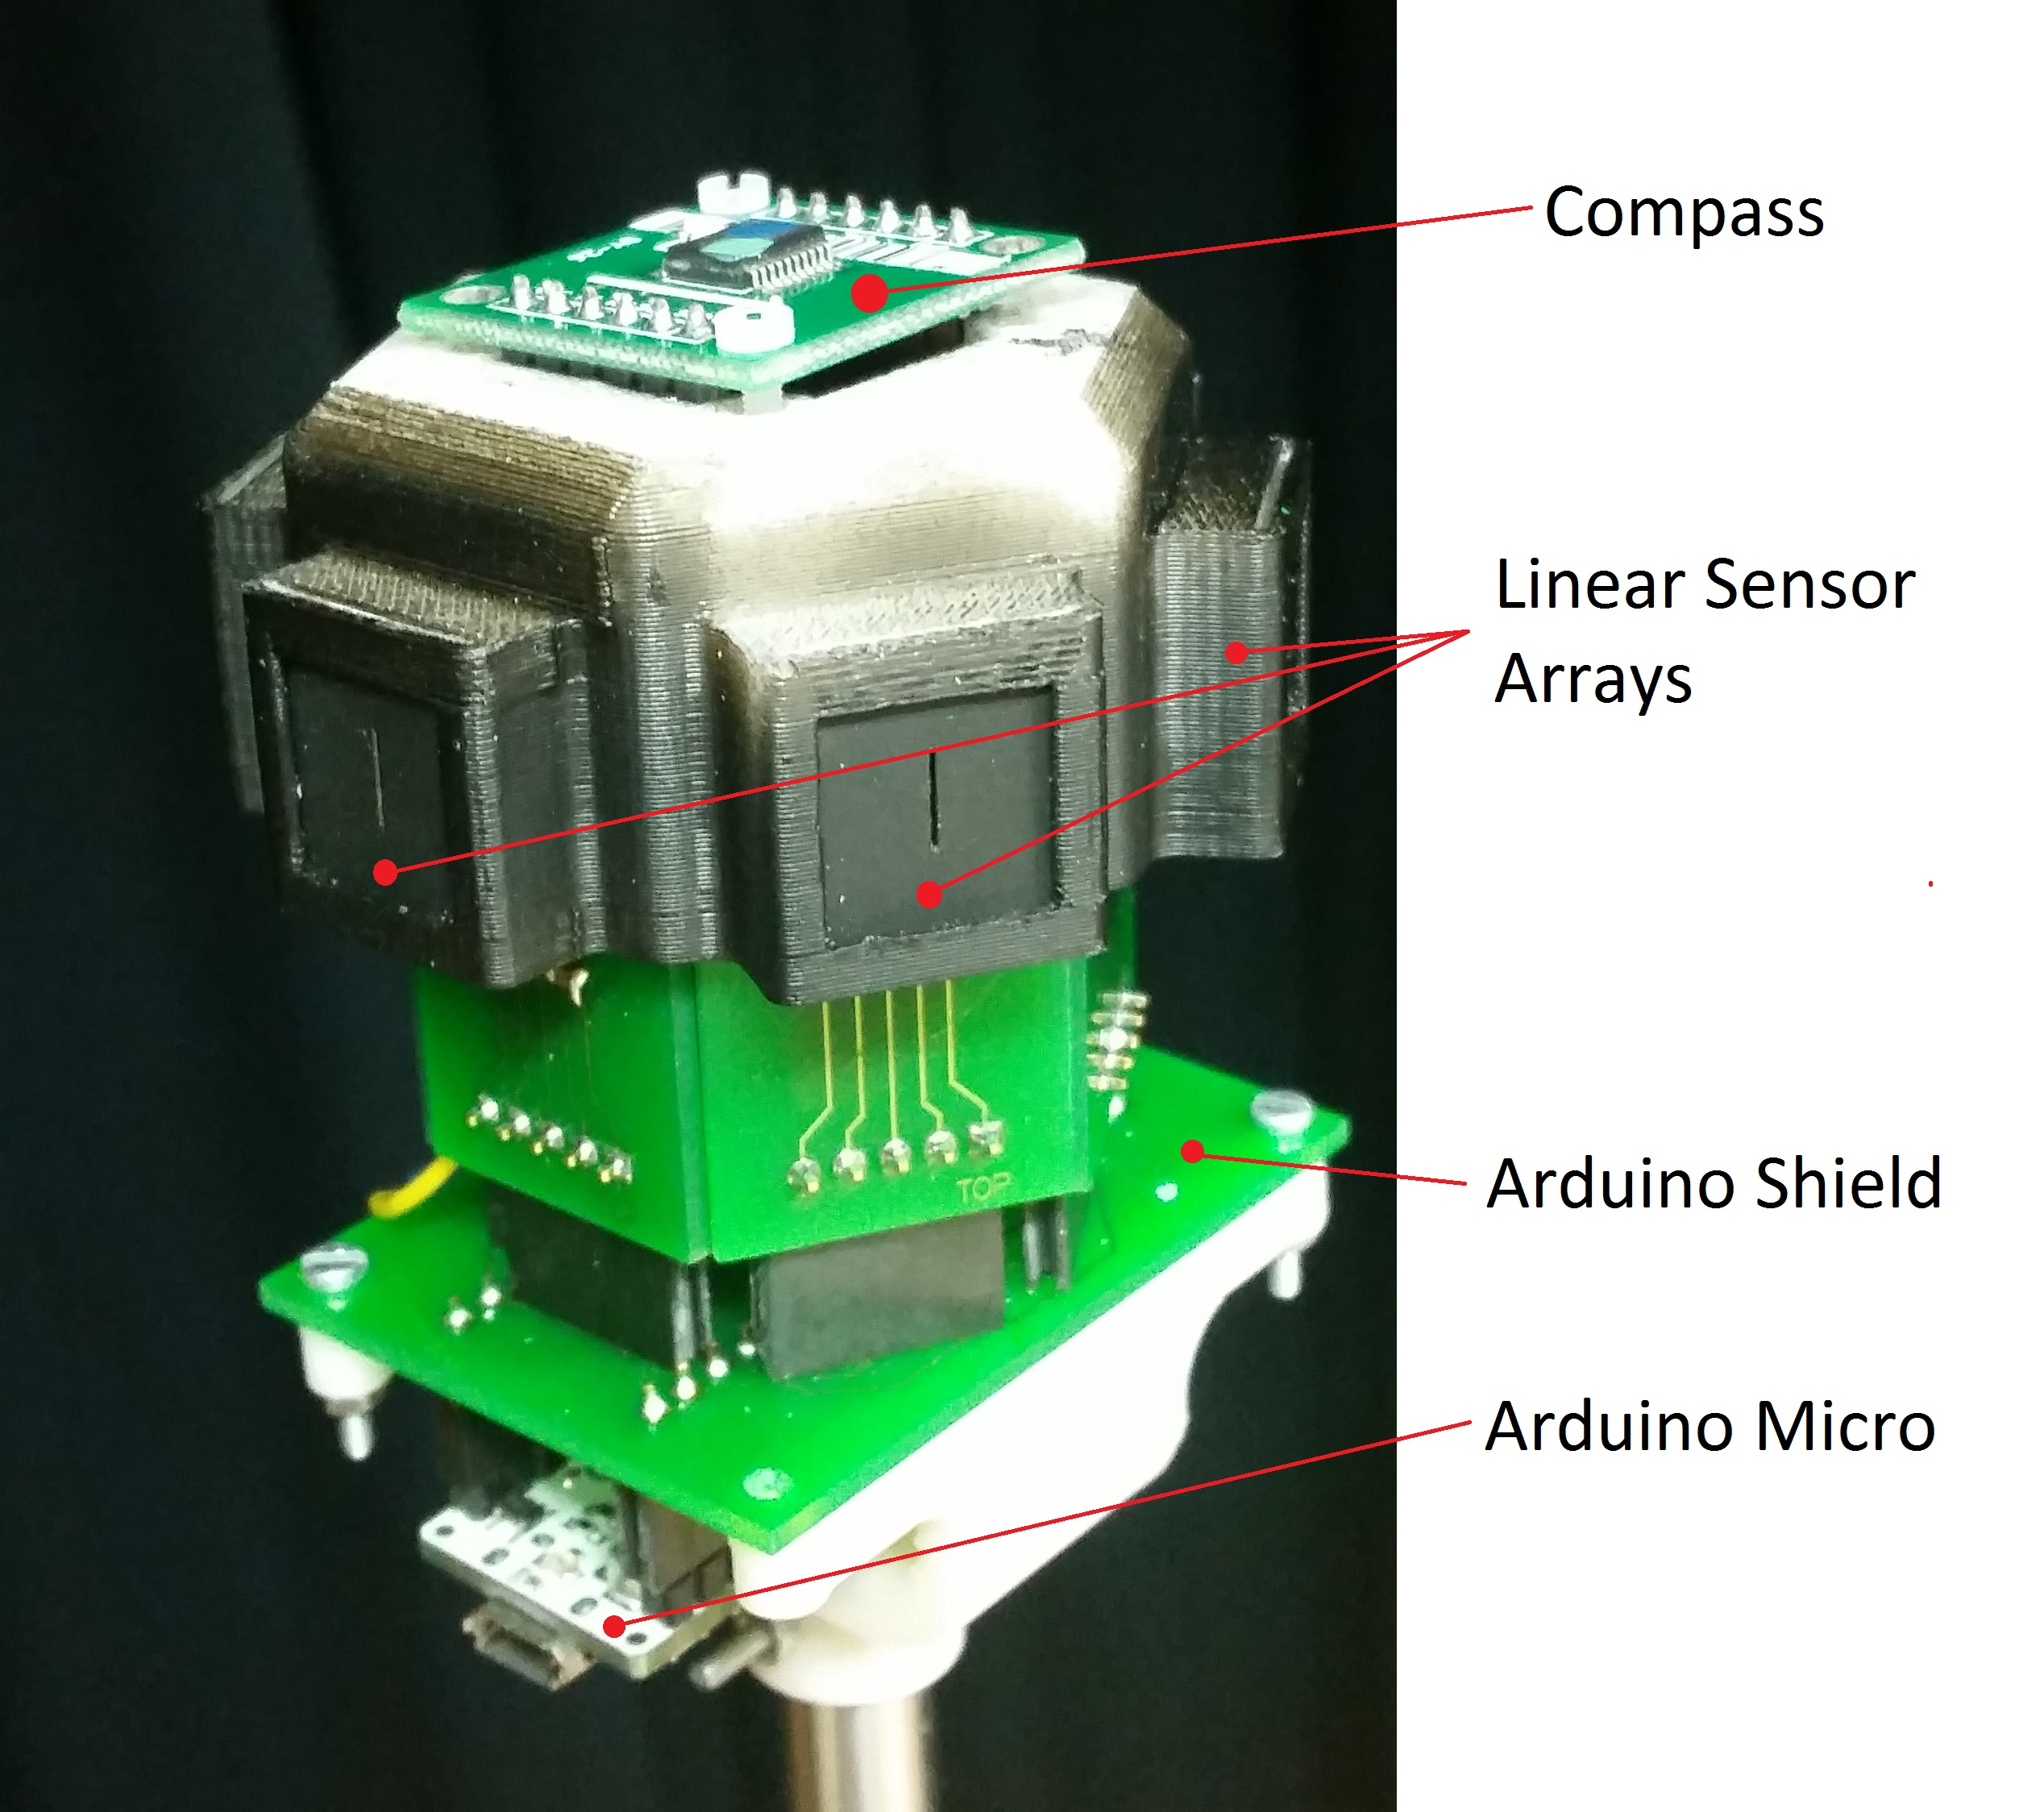
\includegraphics[width=0.5\textwidth]{lincam.jpg}
\caption{The localization module.}
\label{fig:lincam}
\end{figure}

\subsection{Sensors}
Data from two different sensor types are fused to obtain the robot's pose 
(position and orientation) in the arena. A digital compass and an array of
six linear cameras

\subsubsection{Compass}
The compass directly returns the orientation in a range from $0.0^\circ$ and $360.0^\circ$.
Pose updates are queried once per iteration. The purpose of this sensor is to 
give absolute orientation estimates in any place of the arena and independently of
occlusions. In the arena, the compass was also calibrated at the initialization of the program, in order to have a fixed north, pointing at the robot starting orientation.

\subsubsection{Linear Cameras}
The heart of our localization module is formed by six linear cameras arranged 
as a hexagon. All pixel arrays have the same height and inclination, which allows
us to make the simplifying assumption that an image stitched together from all the
cameras captures a $360^\circ$-scene and can be mapped to a circle. Missing pixels
in gaps between, cameras and also the fact that the arrays are not exactly circular
but piecewise planar, are ignored in the following.

Given that there are four light beacons attached to the corners of the arena a 
2D position can be computed from the intensity peeks in the camera image.
This setup could technically be used as a standalone module to determine orientation
and position even without compass (if an initial pose is known). However, a compass 
adds valuable redundancy and especially allows for accurate orientation measurement
in any location inside the arena whereas the achievable accuracy of triangulated 
values through the camera signal varies strongly within the arena due to occlusions
or distant light beacons.

\subsection{Localization algorithm}
Each camera is equipped with a linear image sensor of length 102 and depth 255. This
yields a total of 612 pixels on the whole circle. Mapping pixels to degrees causes a 
resolution of approximately two pixels per degree. An exact determination of peeks 
representing the four light beacons is difficult for two main reasons: firstly, there may be
reflections causing false negatives and secondly, there will be at most three beacons
seen at a time since the fourth one is occluded by the elevated zone of the arena.
Both cases cause ambiguities that would have to be resolved in a bottom-up approach
where one tries to infer position from image peeks. To deal with this difficulty,
we designed a top-down algorithm that follows the idea of expectation maximization.

General:
\begin{itemize}
    \item coordinate origins are in the corner of the recycling zone
    \item global orientation of arena is known (rotation of coordinate systems
        between localization module and arena is determined by compass)
\end{itemize}

In a prior consideration, the arena is divided into equally spaced squares. The area
of $8m \times 8m$ is sub-sampled in steps of $0.5m$, giving $15 \times 15$ discrete 
positions (walls are excluded). For this limited number of points, we pre-compute 
the expected position of beacon images in the pixel array. The result is stored in
\texttt{char prior[15][15][4]}. Dimensions one and two refer to the $x$- and $y$-coordinates.
The third refers two the beacon index.

Consider Algorithm~\ref{alg:localize}. Instead of searching for peeks in the signal 
and estimating our position by triangulation,
we reduce location updates to a weighted average of four pre-computed sampling points.


\begin{algorithm}
\caption{Position update.}
\label{alg:localize}
\begin{algorithmic}[1]
    \Statex Given: initial position $\vec{p_t} = (x_t, y_t)$, camera image $I$, prior[x][y][idx], mapping from angle to pixel index
    \Statex compute new position $\vec{p_{t+1}}$ as
    \Statex 
    
    \State $\theta \gets$ angular measurement from compass
    \Statex

    \Statex determine current tile and use known sampling points
    \State $\vec{s_{00}} \gets (x, y)$ of left, bottom
    \State $\vec{s_{10}} \gets (x, y)$ of right, bottom
    \State $\vec{s_{11}} \gets (x, y)$ of right, top
    \State $\vec{s_{01}} \gets (x, y)$ of left, top
    \Statex
    
    \Statex compute weights of neighboring samples given the actual intensity response as
    \ForAll{$\vec{p_{xy}}$} 
        \State $w_{xy} = \sum_{i = 0}^4 I(prior[x][y][i] + angleToPixel(\theta))$
    \EndFor
    \Statex 

    \Statex new position as weighted average of known samples
    \State $\vec{p_{t + 1}} = \frac{w_{00} \cdot \vec{s_{00}} 
            + w_{01} \cdot \vec{s_{01}} 
            + w_{11} \cdot \vec{s_{11}}
            + w_{10} \cdot \vec{s_{10}}}
            {w_{00} + w_{10} + w_{11} + w_{01}}$ 

\end{algorithmic}
\end{algorithm}

Given an initial position, we know which sampling points to consider. The prior
tells us where to expect peeks in the image signal. Sample points gain more impact
on pose estimates if they match the expectation more, i.e. have high intensity values 
close to the predicted indexes of beacon images. Knowing an approximate location
lets us rule out all ambiguities that might arise from occlusions or false positives.
A pre-processing step where the circular intensity signal is convolved with a box
filter (sliding average) will widen the peeks and thereby make predictions more
reliable. If the peeks were too distinct and close to Dirac impulses our prior 
is more likely to fail.

\begin{figure}[H]
\centering
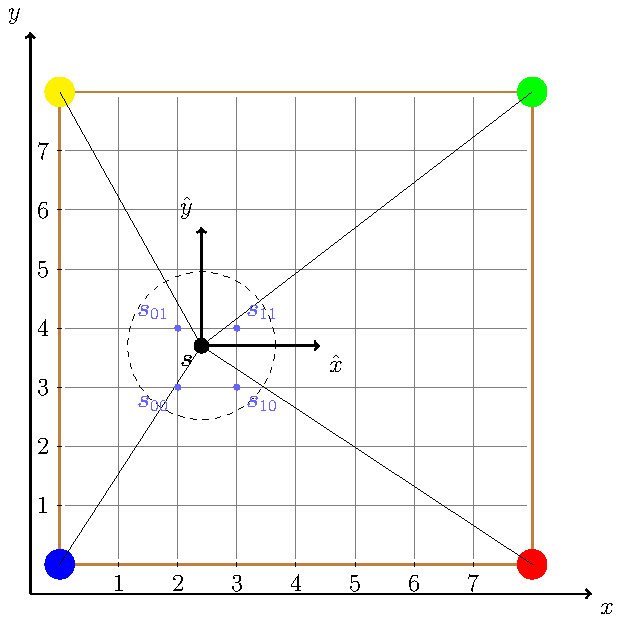
\includegraphics[width=0.5\textwidth]{figures/fig_localization_grid.pdf}
\caption{Exact location $\vec{s}$ and the four closest sampling points. Robot coordinate system is aligned with the arena (no rotation).}
\label{fig:localization_grid}
\end{figure}

% TODO place somewhere else in text
\figurename~\ref{fig:localization_grid} shows the four beacons in the corners of the map, the coordinate system used, and the robot's position.

We want to determine the robots exact
location $\vec{s}$. From previous measurements, we know that we are in the tile
bounded by $\{\vec{s_{00}},\vec{s_{10}},\vec{s_{11}},\vec{s_{01}}\}$. For each 
neighboring sample point, we find the intensity values at the pixel indexes 
predicted by this point (check prior at $\vec{s_{ij}}$ for the needed pixel indexes).
For each $\vec{s_{ij}}$ we then receive a vector of four intensity values. 
Based on the intensities, we compute weights for each sample point. A weighted 
average of  $\{\vec{s_{00}},\vec{s_{10}},\vec{s_{11}},\vec{s_{01}}\}$ yields the
final location estimate.
Note that if we are 
close to a sample point then the respective intensities will be higher because the
peaks match the prediction more than if we were further away. Also if a beacon is
occluded, its respective response would be equally low at all the neighboring  
positions. Hence, we can ignore this fact.
The orientation $\theta$ is important to rotate the local coordinate system before
applying the prior, i.e. the predicted peak pixels must be shifted.

In a very abstract manner 
\begin{itemize}
    \item the prior stores angles at which we expect peaks (as pixel indexes)
    \item the compass is needed to rotate/shift the angles from the prior correctly
    \item we sum up over intensities at indexes given by the prior
    \item this gives us a notion of ``how much does the current location match the predicted one''
    \item weighting the nearest neighbor sample points will give a more accurate
    position estimate
\end{itemize}



\subsection{Tests}

In order to visualize the readings of the different sensors, and to test the algorithm performance in the arena, a python script was written. The script shows a visualization of the intensity values of the 612 pixel array obtain by combining the 6 linear cameras. The blue arrow is also the direction obtained by reading the compass.
 before having the arena, we tried visualizing the peaks in ``good'' conditions. In figure \ref{fig:goodpeak}, the peaks are very high, and easily visisble. 

\begin{figure}[H]
\centering
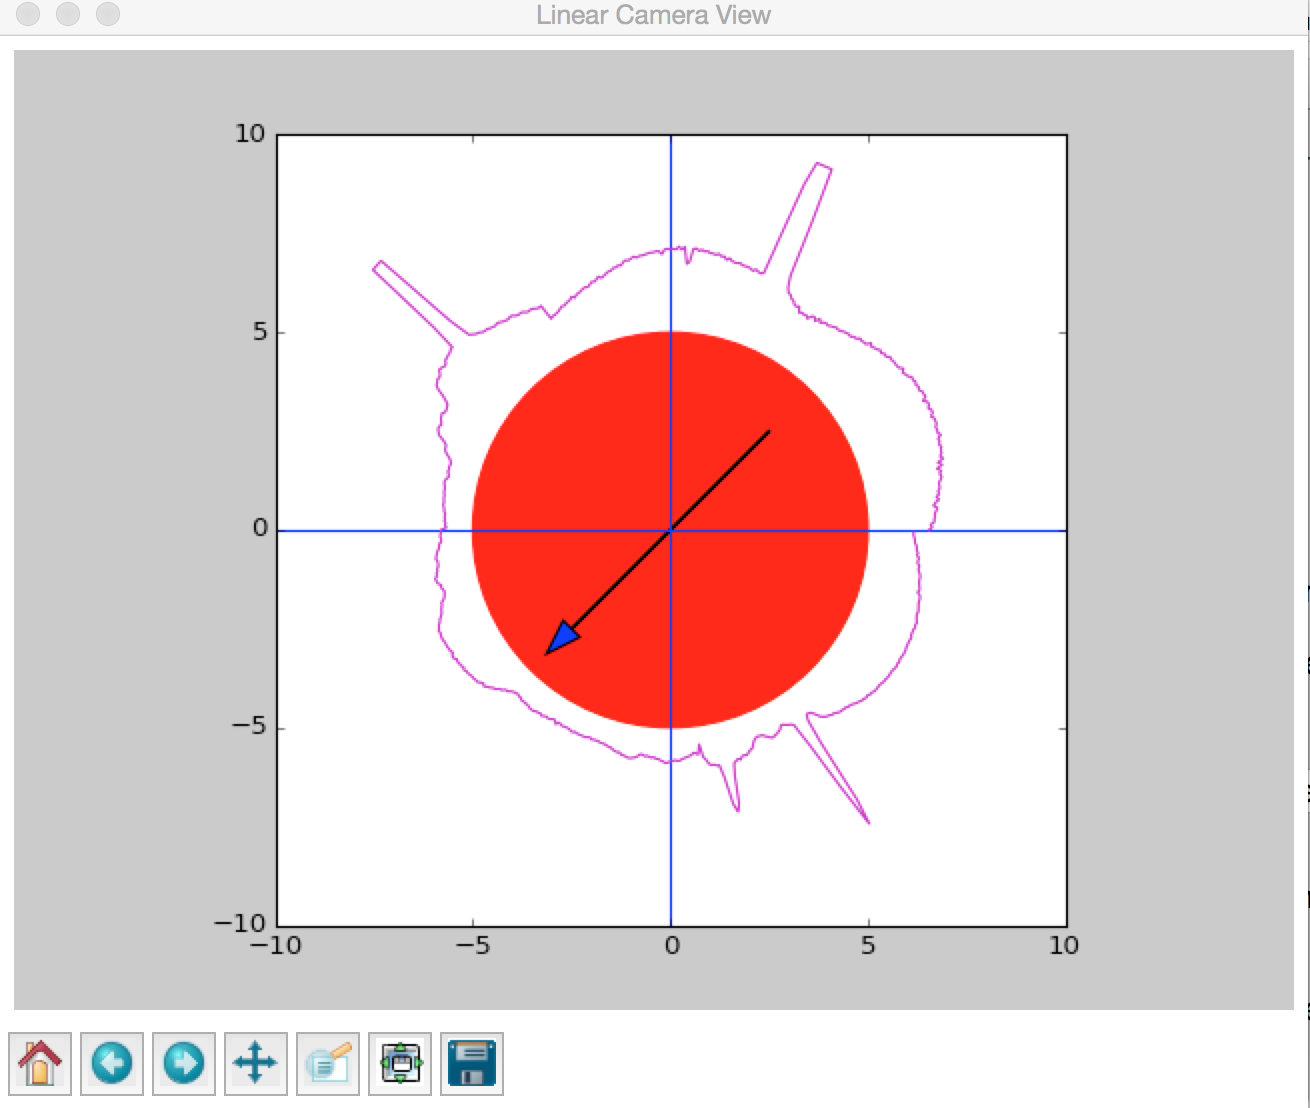
\includegraphics[width=0.5\textwidth]{goodpeak.png}
\caption{Data aquired from the linear sensor arrays in optimal conditions ( low ambient light, high beacon intensity).}
\label{fig:goodpeak}
\end{figure}

With such good conditions, it is easy to find the position of the robot. However, in the real arena, the results were slightly different. In figure \ref{fig:peak}, the real results are shown. As it can be observed, the peak with the highest intensity is coming from one beacon. In this diagram, the robot is very close to the starting position, this is why the intensity is so high. However, the other beacons are barely visible. Some steps can also be observed in the graph, and corresponds to some imperfections of the linear sensor arrays. The sensors were soldered by hand and may not be perfectly flat on the PCB.

\begin{figure}[H]
\centering
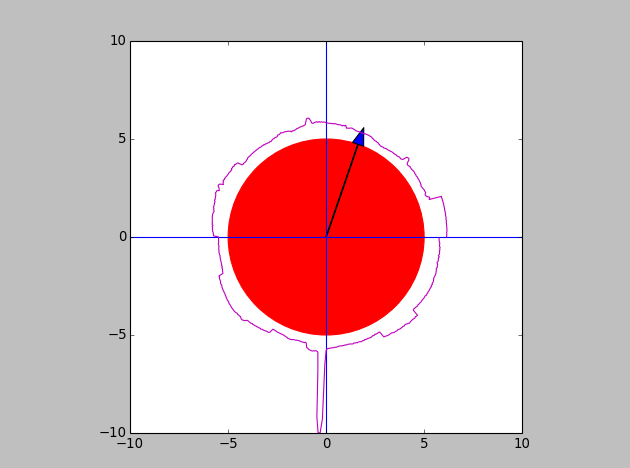
\includegraphics[width=0.5\textwidth]{peak.png}
\caption{Data aquired from the linear sensor arrays in the arena (high ambient light, low beacon intensity).}
\label{fig:peak}
\end{figure}

In the last figure (Figure \ref{fig:roof}), multiple peaks with very high intensity can be seen. These ones corresponds to the roof lights, which are very far. Just by tilting slightly the sensors, ligh pollution begins to appear quite quickly.

\begin{figure}[H]
\centering
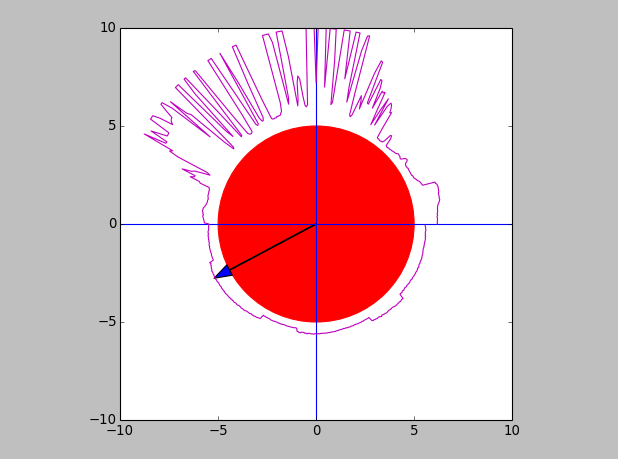
\includegraphics[width=0.5\textwidth]{roof.png}
\caption{Data aquired from the linear sensor arrays in when aiming at the roof of the arena.}
\label{fig:roof}
\end{figure}

Finally, during the competition, we were not able to make the localization work with the beacons, and we used only the compass to give to the robot the direction to where the home was. To find when it was home, the robot used the image processing to locate the beacon that would give a distance towards the recycling area.